\documentclass[12pt, a4paper, oneside]{ctexart}
\usepackage{amsmath, amsthm, amssymb, bm, color, graphicx, geometry, mathrsfs,extarrows, braket, booktabs, array}
\usepackage[colorlinks,linkcolor=red,anchorcolor=blue,citecolor=blue,urlcolor=blue,menucolor=black]{hyperref}
%%%% 设置中文字体 %%%%
\setCJKmainfont{方正新书宋_GBK.ttf}[ BoldFont = 方正小标宋_GBK, ItalicFont = 方正楷体_GBK]
%%%% 设置英文字体 %%%%
\setmainfont{Times New Roman}
\setsansfont{Calibri}
\setmonofont{Consolas}

\linespread{1.4}
%\geometry{left=2.54cm,right=2.54cm,top=3.18cm,bottom=3.18cm}
\geometry{left=1.84cm,right=1.84cm,top=2.18cm,bottom=2.18cm}
\newcounter{problem}  % 问题序号计数器
\newenvironment{problem}{\stepcounter{problem}\par\noindent\textbf{题目\arabic{problem}. }}{\smallskip\par}
\newenvironment{solution}[1]{\par\noindent\textbf{#1解答. }}{\smallskip\par}
\newenvironment{note}{\par\noindent\textbf{注记. }}{\smallskip\par}

\usepackage{minted}
\renewcommand{\theFancyVerbLine}{
    \sffamily\textcolor[rgb]{0.5,0.5,0.5}{\scriptsize\arabic{FancyVerbLine}}} % 修改代码前序号大小
\newmintinline{python}{linenos, breaklines, frame=lines, python3}  % 使用\pythoninline{代码}
\newmintinline{cpp}{linenos, breaklines, frame=lines}  % 使用\c++inline{代码}
\newminted{python}{linenos, breaklines, frame=lines, python3}  % 使用\begin{pythoncode}代码\end{pythoncode}
\newminted{cpp}{fontsize=\small, linenos, breaklines, frame=lines}  % 使用\begin{pythoncode}代码\end{pythoncode}
\newmintedfile{python}{linenos, breaklines, frame=lines, python3}  % 使用\pythonfile{代码地址}

%%%% 图片相对路径 %%%%
\graphicspath{{figure/}} % 当前目录下的figure文件夹, {../figure/}则是父目录的figure文件夹

\everymath{\displaystyle} % 默认全部行间公式
\DeclareMathOperator*\uplim{\overline{lim}} % 定义上极限 \uplim_{}
\DeclareMathOperator*\lowlim{\underline{lim}} % 定义下极限 \lowlim_{}
\let\leq=\leqslant % 将全部leq变为leqslant
\let\geq=\geqslant % geq同理

%%%% 一些宏定义 %%%%
\def\bd{\boldsymbol}        % 加粗(向量) boldsymbol
\def\disp{\displaystyle}    % 使用行间公式 displaystyle(默认)
\def\tsty{\textstyle}       % 使用行内公式 textstyle
\def\sign{\text{sign}}      % sign function
\def\wtd{\widetilde}        % 宽波浪线 widetilde
\def\R{\mathbb{R}}          % Real number
\def\N{\mathbb{N}}          % Natural number
\def\Z{\mathbb{Z}}          % Integer number
\def\Q{\mathbb{Q}}          % Rational number
\def\C{\mathbb{C}}          % Complex number
\def\d{\mathrm{d}}          % differential operator
\def\e{\mathrm{e}}          % Euler's number
\def\i{\mathrm{i}}          % imaginary number
\def\re{\mathrm{Re}}        % Real part
\def\im{\mathrm{Im}}        % Imaginary part
\def\res{\mathrm{Res}}      % Residue
\def\L{\mathcal{L}}         % Loss function
\def\O{\mathcal{O}}         % 时间复杂度
\def\wdh{\widehat}          % 宽帽子 widehat
\def\ol{\overline}          % 上横线 overline
\def\ul{\underline}         % 下横线 underline
\def\add{\vspace{1ex}}      % 增加行间距
\def\del{\vspace{-3.5ex}}   % 减少行间距

%%%% 定理类环境的定义 %%%%
\newtheorem{theorem}{定理}

%%%% 基本信息 %%%%
\newcommand{\RQ}{\today} % 日期
\newcommand{\km}{算法设计与分析} % 科目
\newcommand{\bj}{强基数学002} % 班级
\newcommand{\xm}{吴天阳} % 姓名
\newcommand{\xh}{2204210460} % 学号

\begin{document}

%\pagestyle{empty}
\pagestyle{plain}
\vspace*{-15ex}
\centerline{\begin{tabular}{*5{c}}
    \parbox[t]{0.25\linewidth}{\begin{center}\textbf{日期}\\ \large \textcolor{blue}{\RQ}\end{center}} 
    & \parbox[t]{0.25\linewidth}{\begin{center}\textbf{科目}\\ \large \textcolor{blue}{\km}\end{center}}
    & \parbox[t]{0.2\linewidth}{\begin{center}\textbf{班级}\\ \large \textcolor{blue}{\bj}\end{center}}
    & \parbox[t]{0.1\linewidth}{\begin{center}\textbf{姓名}\\ \large \textcolor{blue}{\xm}\end{center}}
    & \parbox[t]{0.15\linewidth}{\begin{center}\textbf{学号}\\ \large \textcolor{blue}{\xh}\end{center}} \\ \hline
\end{tabular}}
\begin{center}
    \zihao{3}\textbf{第二次作业}
\end{center}\vspace{-0.2cm}
% 正文部分
\begin{solution}{(2-7)}
    设$P_d(x) = (x-n_1)(x-n_2)\cdots(x-n_d)$,其满足$P(n_1)=P(n_2)=\cdots=P(n_d)=0$且最高次项为$1$的$d$次的多项式,考虑使用分治法对其进行计算,不妨令$d = 2^k$,利用递归式$P_d(x) = P_{d/2}(x)\cdot Q_{d/2}(x)$,其中$P_{d/2}(x) = (x-n_1)(x-n_2)\cdots(x-n_{2^{k-1}}),\ Q_{d/2}(x) = (x-n_{2^{k-1}+1})(x-n_{2^{k-1}+2})+\cdots(x-n_{2^{k}})$. 则时间复杂度为
    \begin{align*}
        T(d) =&\ \frac{d}{2}\times 1+\frac{d}{2^2}\times 2\log 2+\cdots+\frac{d}{2^k}\times 2^{k-1}\log 2^{k-1}\\
        =&\ \frac{d}{2}(1+1+2+3+\cdots+k-1) = \O\left(\frac{d}{2}\left(\frac{k(k-1)}{2}+1\right)\right) = \O(d\log^2d).
    \end{align*}
\end{solution}
\begin{solution}{(2-9), (2-10)}
    若数组中存在主元$a$,令$k = \lceil\log x\rceil$,当$n$为奇数时,至少必有以下两种情况之一($n$为偶数时,只会出现情况一):
    
    1. 主元在$T[0\sim n-2]$中,则必有至少三个相同项相邻且为主元,于是可通过以下递归算法查找主元. 存在$i_0\in [1, \lfloor n/2\rfloor]$,使得$T[2i_0-1] = T[2i_0]$,所以只需枚举$n/2$项,建立新的数组$Q$,当$T[2i_0-1] = T[2i_0]$时,\add 将下标$2i_0$加入数组$Q$中,再递归地在$Q$中找主元. 时间复杂度为$\O\left(n\left(\frac{1}{2}+\frac{1}{2^2}+\cdots+\frac{1}{2^k}\right)\right) = \O(n-1)$.\add

    2. 主元为$T[n-1]$,\add 可以直接通过遍历整个数组判断该元素是否是主元. 结合第一种递归,则时间复杂度为$\O\left(n\left(1+\frac{1}{2}+\cdots+\frac{1}{2^{k-1}}\right)\right)) = \O(2n-1)$\add

    综上,该算法的总时间复杂度为$\O(n)$.

    以下为算法部分,\cppinline{check(x,y)}用于交互查询\cppinline{a[x]}是否与\cppinline{a[y]}相等,其他函数只能通过调用该函数进行查询.
    \begin{cppcode}
#include <cstdio>
#include <vector>
using namespace std;
int a[] = {1, 1, 5, 5, 1, 5, 1};  // 有主元
// int a[] = {1, 1, 5, 5, 1, 5};  // 没有主元
// int a[] = {1, 1, 5, 5, 1, 1};  // 有主元
// int a[] = {1, 3, 2, 5, 1, 5, 1};  // 没有主元
bool check(int x, int y) {
    // 这个就是交互用的,专门用于返回a[x],a[y]是否相等,
    // 其他函数只能通过该函数访问数组
    return a[x] == a[y];
}
// v存储当前可能是主元的下标
bool find(vector<int> v) {  // 只能通过下标数组判断
    int n = v.size();
    if (n == 0) {
        return false;
    }
    vector<int> Q;
    for (int i = 1; i < n; i += 2) {
        if (check(v[i-1], v[i])) {
            Q.push_back(v[i]);
        }
    }
    if (n % 2 == 1) {
        int cnt = 1;
        for (int i = 0; i < n-1; i++) {
            if (check(v[i], v[n-1])) {
                cnt++;
            }
        }
        if (cnt > n/2) {
            return true;
        }
    }
    return find(Q);
}
int main() {
    int n = sizeof(a) / sizeof(int);
    vector<int> v;  // 需要判断的下标数组
    for (int i = 0; i < n; i++) {
        v.push_back(i);
    }
    if (find(v)) {
        printf("有主元\n");
    } else {
        printf("没有主元\n");
    }
}
    \end{cppcode}
\end{solution}
\clearpage
\begin{solution}{(2-28)}
    通过由于两个数组都是有序数组,可通过二分法查找中位数,假设当前第一个数组的查找范围为$[l_1,r_1)$中位数为$mid_1$,第二个枚举范围为$[l_2,r_2)$中位数为$mid_2$,分三种情况:

    1. 若$mid_1 < mid_2$,则进一步递归查找,第一个数组查找范围为$\left[\frac{l_1+r_2}{2}, r_1\right)$第二个数组查找范围为$\left[l_2,\frac{l_2+r_2}{2}\right)$.

    2. 若$mid_1 > mid_2$,则进一步递归查找,第一个数组查找范围为$\left[l_1, \frac{l_1+r_2}{2}\right)$第二个数组查找范围为$\left[\frac{l_2+r_2}{2}, r_2\right)$.\add

    3. 若$mid_1 = mid_2$,则找到公共中位数返回$mid_1$.

    边界条件:若没有第三种返回条件,则最终会遍历到数组的边界,直接返回两个数组端点值的均值. 故时间复杂度为$\O(\log n)$.

    注:上述除法均为向下取整.
    \begin{cppcode}
#include <bits/stdc++.h>
using namespace std;
int a[] = {1,2,3,4,5};  // 中位数为3.5
int b[] = {3,4,5,6,7};
// int a[] = {1,2,3,4,5};  // 中位数为5.5
// int b[] = {6,7,8,9,10};
// int a[] = {3,4,5,6,7};  // 中位数为3.5
// int b[] = {1,2,3,4,5};

double calc_mid(int *a, int l, int r) { // 计算数组a[l~r]的中位数
    int k = (l + r) / 2;
    if ((r - l + 1) % 2 == 0) {
        return (a[k] + a[k+1]) / 2.0;
    } else {
        return a[k];
    }
}
double get_mid(int l1, int r1, int l2, int r2) {
    if (l1 == r1-1) {  // 枚举到端点,中位数在两个数组之间
        return (a[l1] + b[l2]) / 2.0;
    }
    double mid1 = calc_mid(a, l1, r1);
    double mid2 = calc_mid(b, l2, r2);
    if (abs(mid1 - mid2) < 1e-6) {
        return mid1;
    }
    if (mid1 < mid2) {
        return get_mid((l1+r1)/2, r1, l2, (l2+r2)/2);
    } else return get_mid(l1, (l1+r1)/2, (l2+r2)/2, r2);
}

int main() {
    int n = sizeof(a) / sizeof(int);
    printf("中位数为%.2f\n", get_mid(0, n, 0, n));
    return 0;
}
    \end{cppcode}
\end{solution}

% 下面给一些功能的写法
\iffalse
% 图片模板
\centerline{
    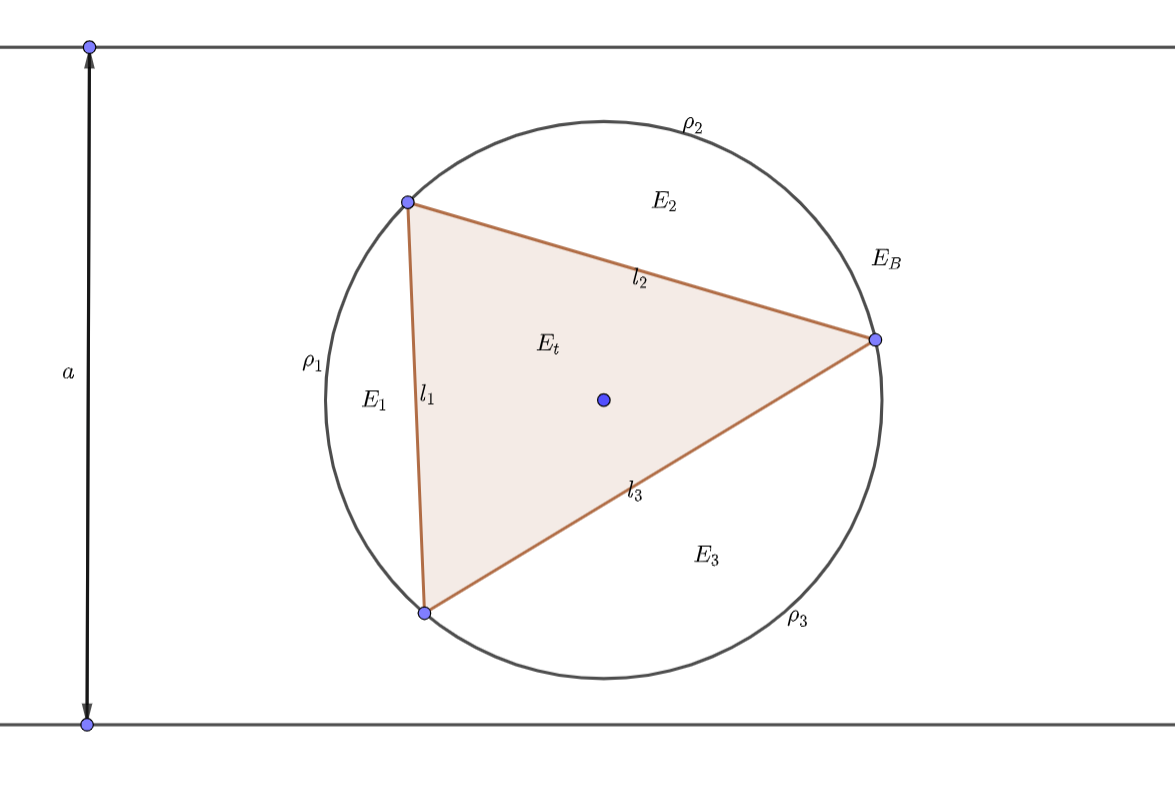
\includegraphics[width=0.8\textwidth]{figure.png}
}
% 表格模板
\renewcommand\arraystretch{0.8} % 设置表格高度为原来的0.8倍
\begin{table}[!htbp] % table标准
    \centering % 表格居中
    \begin{tabular}{p{1cm}<{\centering}p{1cm}<{\centering}p{3cm}<{\centering}p{5cm}<{\centering}} % 设置表格宽度
    %\begin{tabular}{cccc}
        \toprule
        $x_i$ & $f[x_1]$ & $f[x_i,x_{i+1}]$ & $f[x_i,x_{i+1},x_{i+2}]$ \\
        \midrule
        $x_0$ & $f(x_0)$ &                  &                          \\
        $x_0$ & $f(x_0)$ & $f'(x_0)$        &                          \\
        $x_0$ & $f(x_1)$ & $\frac{f(x_1)-f(x_0)}{x_1-x_0}$ & $\frac{f(x_1)-f(x_0)}{(x_1-x_0)^2}-\frac{f'(x_0)}{x_1-x_0}$\\
        \bottomrule
    \end{tabular}
\end{table}

\def\Log{\text{Log}} % 一个简单的宏定义
$\Log$ % 调用方法
\fi

\end{document}